\documentclass[14pt,a4paper]{extarticle}
\usepackage[T1]{fontenc}
\usepackage[utf8]{inputenc}
\usepackage[scaled]{helvet}
\renewcommand{\familydefault}{\sfdefault}
\usepackage{amsmath}
\usepackage{sansmath}
\sansmath
\usepackage[a4paper,margin=2cm]{geometry}
\usepackage{tikz}
\usetikzlibrary{angles,quotes,patterns}
\usepackage{array}
\pagestyle{empty}
% Zweite Seite: 5-mm-Kästchen, 1 cm Rand
\newcommand{\kaestchen}{\newpage\null\begin{tikzpicture}[remember picture,overlay]
\begin{scope}[shift={(current page.south west)}]\draw[step=5mm, black!45, line width=0.3pt] (1cm,1cm) grid (20cm,28.5cm);\draw[black!45, line width=0.3pt] (1cm,1cm) rectangle (20cm,28.5cm);\end{scope}
\end{tikzpicture}}
\setlength{\parindent}{0pt}
\hyphenpenalty=10000

% Nur Schwarz und Grau, die Blätter werden schwarz-weiß kopiert.
% Merkblock: Begriff und Text links, Zeichnung rechts.
\newcommand{\bl}{0.5}
\newcommand{\block}[3]{%
\begin{minipage}[c]{\bl\textwidth}\raggedright{\Large\bfseries #1\par}\medskip #2\end{minipage}\hfill
\begin{minipage}[c]{\dimexpr0.97\textwidth-\bl\textwidth\relax}\centering #3\end{minipage}\par}

\renewcommand{\bl}{0.46}
\begin{document}

{\LARGE\bfseries Mittelsenkrechte und Winkelhalbierende\par}
\vspace{0.9cm}

\block{Mittelsenkrechte}{%
Jeder Punkt auf der Mittelsenkrechten von $AB$ ist von $A$ und $B$ gleich weit entfernt. Sie geht durch die Mitte $M$ von $AB$ und steht senkrecht auf $AB$.\par\medskip
\begin{tabular}{@{}l@{\ }>{\raggedright\arraybackslash}p{0.88\linewidth}@{}}
1. & Kreis um $A$, Radius mehr als die halbe Strecke\\
2. & Kreis um $B$ mit gleichem Radius\\
3. & Gerade durch die beiden Schnittpunkte
\end{tabular}\par\medskip
Mit dem Geodreieck: Mitte von $AB$ messen, Senkrechte durch $M$ zeichnen.}{%
\begin{tikzpicture}[scale=2.4]
  \draw[gray, thick, dashed] (25:2) arc (25:57:2); \draw[gray, thick, dashed] (-25:2) arc (-25:-57:2);
  \draw[gray, thick, dashed] ([shift={(3,0)}]155:2) arc (155:123:2); \draw[gray, thick, dashed] ([shift={(3,0)}]205:2) arc (205:237:2);
  \draw[very thick] (1.5,-1.9) -- (1.5,1.9);
  \draw (1.75,0) arc (0:90:0.25); \fill (1.5,0) ++(45:0.11) circle (1pt);
  \draw[thick] (0,0) -- (3,0);
  \fill (0,0) circle (1.6pt) node[left] {$A$}; \fill (3,0) circle (1.6pt) node[right] {$B$}; \fill (1.5,0) circle (1.6pt) node[below right] {$M$};
\end{tikzpicture}}

\vspace{1cm}

\block{Winkelhalbierende}{%
Jeder Punkt auf der Winkelhalbierenden ist von beiden Schenkeln gleich weit entfernt. Sie teilt den Winkel in zwei gleich große Teile.\par\medskip
\begin{tabular}{@{}l@{\ }>{\raggedright\arraybackslash}p{0.88\linewidth}@{}}
1. & Kreis um $S$, er schneidet beide Schenkel\\
2. & Um beide Schnittpunkte je ein Kreis mit gleichem Radius\\
3. & Gerade von $S$ durch den neuen Schnittpunkt
\end{tabular}\par\medskip
Mit dem Geodreieck: Winkel messen, halbieren, Hälfte antragen.}{%
\begin{tikzpicture}[scale=2.0]
  \draw[gray, thick, dashed] (-8:1.5) arc (-8:78:1.5);
  \draw[gray, thick, dashed] ([shift={(1.5,0)}]55:1.5) arc (55:85:1.5);
  \draw[gray, thick, dashed] ([shift={(0.513,1.410)}]-15:1.5) arc (-15:15:1.5);
  \draw[very thick] (0,0) -- (35:3.6);
  \draw[thick] (0,0) -- (4,0); \draw[thick] (0,0) -- (70:3.3);
  \fill (0,0) circle (1.6pt) node[left] {$S$};
  \node at (17.5:1.12) {$35^\circ$}; \node at (52.5:1.12) {$35^\circ$};
\end{tikzpicture}}

\vspace{1cm}

{\Large\bfseries Aufgaben im Heft\par}
\medskip
Buch S.\,\rule{1.5cm}{0.4pt} Nr.\,\rule{5cm}{0.4pt}

\kaestchen
\end{document}
